\documentclass[t,10pt]{beamer}
\beamertemplatenavigationsymbolsempty

\definecolor{GitRed}{RGB}{240, 60, 46}
\setbeamercolor{title}{bg=GitRed,fg=white}
\setbeamercolor{structure}{fg=black}
\setbeamertemplate{section in toc shaded}[default][40]
\setbeamercolor{itemize item}{fg=GitRed}
\setbeamercolor{section in toc}{bg=GitRed,fg=white}
\setcounter{tocdepth}{1}
\setbeamertemplate{section in toc}{\inserttocsectionnumber.~\inserttocsection}

% allow copy & paste, make nice tilde
\usepackage[T1]{fontenc}
% do not use bitmap font
\usepackage{lmodern}

% Quotations
\usepackage{epigraph}
\setlength\epigraphwidth{10cm}
\setlength\epigraphrule{0pt}
\renewcommand{\epigraphsize}{\normalsize}
%\usepackage{etoolbox}
%\makeatletter
%\patchcmd{\epigraph}{\@epitext{#1}}{\itshape\@epitext{#1}}{}{}
%\makeatother

\usepackage{url}
\usepackage{relsize}
\usepackage{hyperref}
\hypersetup{colorlinks=true, urlcolor=structure.fg, linkcolor=structure.fg}
\renewcommand*{\UrlFont}{\ttfamily\footnotesize\relax}

%\usepackage{bold-extra} % cmtt
%\renewcommand{\ttdefault}{cmtt}
%\usepackage{lmodern}
%\usepackage{pxfonts}  % Palatino font
%%\usepackage{txfonts}  % Times font

\makeatletter
\newcommand\handoutmode[1]{
  \ifnum1=0#1
    \gdef\beamer@currentmode{handout}
    \usepackage{../handoutWithNotes}
    \pgfpagesuselayout{4 on 1}[a4paper, landscape, border shrink=5mm]
    \setbeamertemplate{navigation symbols}{}
    \setbeamertemplate{headline}{%
      \leavevmode%
      \vspace{.5cm}
    }



    % define font of lstlisting
    \lstset{
      basicstyle=\small\ttfamily\bfseries, %\tiny\ttfamily,
      tabsize=2,
      extendedchars=true,
      breaklines=true,
      %frame=single,
      %stringstyle=\ttfamily,
      showspaces=false,
      showtabs=false,
      xleftmargin=.25cm,
      %framextopmargin=0pt,
      %framexleftmargin=2pt,
      %framexrightmargin=2pt,
      %framexbottommargin=0pt,
      backgroundcolor=\color{white},
      showstringspaces=false
      %morestring=[b][\color{blue}]",
      %morestring=[d][\color{blue}]',
      columns=fullflexible,
      escapeinside={(*}{*)},
      keepspaces=true,
      upquote=true,
      commentstyle=\color{red},
      keywordstyle=\color{blue},
      rulecolor=\color{gray}
    %  language=bash
    }
    %\lstloadlanguages{bash}
  \else
    \AtBeginSection[]{
      \begin{frame}<*>{Outline}
        \hspace{1.2em}
        \begin{multicols}{2}
        \frametitle{Outline}
        \tableofcontents[currentsection] %,hideallsubsections]
        \end{multicols}
      \end{frame}
    }
    \addtocontents{toc}{\vskip -0.2cm}
    \setbeamertemplate{footline}[text line]{%
      \parbox{\linewidth}{\vspace*{-12pt}\textcolor{lightgray}{\inserttitle{} {\normalsize\ttfamily\textcopyright}\
        Andr\'{e} Roth, Andreas Schmid, Eric Keller - Licensed for: Creative Commons Attribution Share Alike 4.0 International
      \hfill \insertpagenumber/\pageref{LastPage}}}
    }
    \setbeamertemplate{navigation symbols}{}

    \setbeamercolor{title}{fg=white, bg=GitRed}
    \setbeamercolor{frametitle}{fg=white, bg=GitRed}

    \setbeamercolor{section in toc}{fg=black,bg=white}

    \setbeamertemplate{frametitle}
    {
        \nointerlineskip
        \begin{beamercolorbox}[sep=0.01cm,ht=1.8em,wd=\paperwidth]{frametitle}
          %\vbox{}\vskip-4ex%
          \hspace{.3cm}\strut\textbf\insertframetitle\strut
          %\vskip-0.8ex%
          \hfill$\vcenter{\hbox{
\includegraphics{assets/diagrams/git-logo-small.pdf}}}$
        \end{beamercolorbox}
    }

    % define font of lstlisting
    \definecolor{listingbackground}{rgb}{0,0,0}
    \lstset{
      basicstyle=\small\ttfamily\bfseries\color{black}, %\tiny\ttfamily,
      tabsize=2,
      extendedchars=true,
      breaklines=true,
      frame=leftline,
      %stringstyle=\ttfamily,
      showspaces=false,
      showtabs=false,
      xleftmargin=.25cm,
      %framextopmargin=0pt,
      %framexleftmargin=2pt,
      %framexrightmargin=2pt,
      %framexbottommargin=0pt,
      backgroundcolor=\color{white},
      showstringspaces=false
      %morestring=[b][\color{blue}]",
      %morestring=[d][\color{blue}]',
      columns=fullflexible,
      escapeinside={(*}{*)},
      keepspaces=true,
      upquote=true,
      commentstyle=\color{red},
      keywordstyle=\color{blue},
      rulecolor=\color{gray}
    %  language=bash
    }
    %\lstloadlanguages{bash}

  \fi
}
\makeatother

\usepackage{catchfile}
\newcommand{\getenv}[2][]{%
  \CatchFileEdef{\temp}{"|kpsewhich --var-value #2"}{}%
  \if\relax\detokenize{#1}\relax\temp\else\let#1\temp\fi}

\usepackage{listings}

\getenv[\HANDOUT]{HANDOUT}
\handoutmode{\HANDOUT}

\usepackage[utf8]{inputenc}
\usepackage{multicol}
\usepackage{color,soul}
\usepackage{tabto}
\usepackage{inconsolata}
\usepackage{graphicx}
\usepackage{wrapfig}
\usepackage{upquote}
\usepackage{vwcol}
\usepackage{lastpage}


% table spacings
\renewcommand{\arraystretch}{1.5}

%\setlength{\parskip}{10pt plus 1pt minus 1pt}

\newcommand{\slidetitle}{\frametitle{\thesection. \secname}\vspace{1em}}
\newcommand{\subslidetitle}{\frametitle{\thesection.\thesubsection\ \subsecname}\vspace{1em}}
\newcommand{\subsubslidetitle}{\frametitle{\thesection.\thesubsection.\thesubsubsection\ \subsubsecname}\vspace{1em}}

\newcommand{\cmd}[1]{\textcolor[HTML]{0000AA}{\texttt{\textbf{#1}}}}
\newcommand{\option}[3][1cm]{\item[]{\usebeamercolor[structure.fg]{section in head}\texttt{#2}}\tabto{#1}#3}
\newcommand{\opt}[3][2cm]{\item{\usebeamercolor[structure.fg]{section in head}\texttt{#2}}\tabto{#1}#3}

\def\braces#1{[#1]}
\def\lbrace#1{[#1}

\newcounter{exercise}
\newenvironment{exercise}[0]
  {\begin{enumerate}\setcounter{enumi}{\theexercise}}
  { \setcounter{exercise}{\theenumi}\end{enumerate}}

% layout of title side
\makeatletter
\setbeamertemplate{title page}
{
  \vspace{.6cm}
  \center 
\includegraphics{assets/diagrams/git-logo-2color.pdf}
  \vbox{}
  \vfill
  \begingroup
    \centering
    \begin{beamercolorbox}[sep=8pt,center]{title}
      \usebeamerfont{title}\bf{\Huge{workshop}}\par%
      \ifx\insertsubtitle\@empty%
      \else%
        \vskip0.25em%
        {\usebeamerfont{subtitle}\usebeamercolor[fg]{subtitle}\insertsubtitle\par}%
      \fi%
    \end{beamercolorbox}%
    \vskip.5em\par
    \begin{beamercolorbox}[sep=8pt,center]{author}
      \usebeamerfont{author}\insertauthor
    \end{beamercolorbox}
  \endgroup
  \vfill
}
\makeatother
% end of layout of title side

\setbeamerfont{author}{size=\smaller}
\setbeamerfont{date}{size=\smaller}

\begin{document}
\title{git workshop}
\author{
  \textbf{Authors} \\
  André Roth \textless{}neolynx@gmail.com\textgreater{}\\
  Andreas Schmid \textless{}ikeark@gmail.com\textgreater{}\\
  Eric Keller \textless{}keller.eric@gmail.com\textgreater{}\\
  \vspace{.4em}
  \textbf{Licensed for:} Creative Commons Attribution Share Alike 4.0 International
  \textbf{Version:} \today
}
%\date{Version: \today}

\frame{\titlepage}

\section{Introduction}
\begin{frame}
  \slidetitle
  The scope of this workshop covers:
  \begin{itemize}
    \item The concepts of git
    \item The usage of git (tool independent)
    \item Understanding git workflows
  \end{itemize}

  \pause
  \vspace{1em}
  Workshop strategy:
  \begin{itemize}
    \item Hands-on workshop on an example project
    \item Learning-by-doing
  \end{itemize}

  \pause
  \vspace{1em}
  Required skills:
  \begin{itemize}
    \item Basic usage of the command line
    \item Use a text editor (Vim)
    \item Type what is written on the slides :)
  \end{itemize}

  \vspace{1em}
  Note: This workshop takes about 4 hours (hopefully!)
\end{frame}

\subsection{History}
\begin{frame}
  \subslidetitle

  \textbf{Version Control Systems (VCS)}
  \pause
  \\
  \begin{tabular}{lp{6cm}r}
    \textbf{1982} & Revision Control System (RCS) & GNU GPL \\
    \pause
    \textbf{1990} & Concurrent Versions System (CVS) & GNU GPL \\
    \pause
    \textbf{1992} & Rational ClearCase & proprietary \\
    \pause
    \textbf{1995} & Perforce  & proprietary \\
    \pause
    \textbf{2000} & Apache Subversion (SVN)  & Apache \\
  \end{tabular}
\end{frame}

\subsection{History}
\begin{frame}
  \subslidetitle
  \textbf{Distributed Version Control Systems (DVCS)}
  \pause
  \\
  \begin{tabular}{lp{6cm}r}
    \textbf{2000} & BitKeeper  & proprietary \\
    \pause
    \textbf{2001} & GNU arch   & GNU GPL \\
    \pause
    \textbf{2003} & Monotone   & GNU GPL \\
    \pause
    \textbf{2005} & git & GNU GPL \\
    \pause
    \textbf{2005} & GNU Bazaar & GNU GPL \\
    \pause
    \textbf{2005} & Mercurial  & GNU GPL \\
    \pause
  \end{tabular}

  Linus Torvalds created git in order to replace BitKeeper which changed the license in 2005.
\end{frame}

\subsection{About git}
\begin{frame}
  \subslidetitle
   The term 'git' is British slang describing a person that is:
  \begin{itemize}
    \item unpleasant
    \item annoying
    \item childish
  \end{itemize}

  \pause
  \epigraph{``I'm an egotistical bastard, and I name all my projects after myself. First Linux, now git.''}
       {--- Linus Torvalds, 2007-06-14}
  \pause
  \epigraph{``Because my hatred of CVS has meant that I see Subversion as being the most pointless project ever started, because the whole slogan for the Subversion for a while was 'CVS done right' or something like that. And if you start with that kind of slogan, there is nowhere you can go. It's like, there is no way to do CVS right.''}
      {--- Linus Torvalds, Google Tech Talk 2007}
\end{frame}

\subsection{About git}
\begin{frame}
  \subslidetitle
  \textbf{Design goals:}
  \pause
  \begin{itemize}
    \item Take Concurrent Versions System (CVS) as an example of what not to do; if in doubt, make the exact opposite decision
    \pause
    \item Support a distributed, BitKeeper-like workflow
    \pause
    \item Very strong safeguards against corruption, either accidental or malicious
    \pause
  \end{itemize}

  \vspace{2em}
  \textbf{Implementation:}
  \\
  \pause
  \begin{tabular}{ll}
    Started: & 2005-04-03 \\
  \pause
    Announced: &2005-04-06 \\
    \pause
    Self Hosting: & 2005-04-07 (4d!) \\
    \pause
    First Multi Branch Merge: & 2005-04-18 (15d!)
  \end{tabular}

\end{frame}


\section{Getting started}
\begin{frame}[fragile]
  \slidetitle

  In this section, we will learn how to:
  \begin{itemize}
    \item Configure git
    \item Clone a git repository
    \item Add a file to a repository
    \item Commit changes
  \end{itemize}
    %A git repository contains a folder called {\bf .git}. There are two option to get a git repository:
%\begin{itemize}
%\item create a new repository using \cmd{git init}
%\item clone an existing git repository using \cmd{git clone}
%\end{itemize}
\end{frame}

\subsection{Configuring git}
\begin{frame}[fragile]
  \subslidetitle
  The global git configuration is stored in \cmd{~/.gitconfig}.
  \\
  \vspace{1em}

  The command \cmd{git config} can used to configure git:
  \begin{lstlisting}
$ (*\textcolor[HTML]{0000AA}{git config --global add user.name "My name"}*)
$ (*\textcolor[HTML]{0000AA}{git config --global add user.email "myemail@git.ch"}*)
  \end{lstlisting}

  Other git settings:
  \begin{lstlisting}[basicstyle=\small\ttfamily\bfseries]
$ (*\textcolor[HTML]{0000AA}{cat ~/.gitconfig}*)
[color]
  diff = auto
  status = auto
  branch = auto
  grep = auto

[alias]
  st = status
  co = checkout
  ci = commit
  br = branch
  l = log --graph --pretty=format:'%C(yellow)%h%C(cyan)%d%Creset %s %C(white)- %an, %ar%Creset'
  ll = log --stat --abbrev-commit

[merge]
  tool = kdiff3
  \end{lstlisting}

\end{frame}

%\subsection{git init}
%\begin{frame}[fragile]
  %\subslidetitle
  %The command \cmd{git init} is used to create a new repository.
  %The following steps create a new repository:
  %\begin{itemize}
  %\item run \cmd{git init} inside your project
    %\begin{itemize}
    %\item creates .git directory
    %\end{itemize}
  %\item Add files to git repository using \cmd{git add .}
  %\item Optional: add .gitignore file
  %\item Run {git commit} for initial commit
    %\begin{itemize}
    %\item creates branch called 'master'
    %\end{itemize}
  %\end{itemize}

  %\begin{lstlisting}
%cd myproject
%git init
%git add .
%git commit
  %\end{lstlisting}
%\end{frame}

\subsection{Clone a git repository}
\begin{frame}[fragile]
  \subslidetitle
  The command \cmd{git clone} is used to download a whole git repository.
  \\
  \vspace{1em}
  Clone the gitmoon repository:
  \begin{lstlisting}
$ (*\textcolor[HTML]{0000AA}{git clone https://github.com/neolynx/gitmoon.git}*)
  \end{lstlisting}

% protocols
%git protocols:
%\begin{itemize}
%\item http[s]
%\item ssh
%\item git
%\item ftp rsync ...
%\end{itemize}

  Let's see what we find ...
  \begin{lstlisting}
$ (*\textcolor[HTML]{0000AA}{cd gitmoon}*)
$ (*\textcolor[HTML]{0000AA}{ls}*)
moon_1024.jpg  moon.html  moon.js  three.min.js
  \end{lstlisting}

  Oh, there is a HTML file !
  \begin{lstlisting}
$ (*\textcolor[HTML]{0000AA}{firefox moon.html \&}*)
  \end{lstlisting}

\end{frame}

\subsection{Show the git status}
\begin{frame}[fragile]
  \subslidetitle
  \begin{lstlisting}
$ (*\textcolor[HTML]{0000AA}{git status}*)
On branch master
Your branch is up-to-date with 'origin/master'.
nothing to commit, working directory clean
  \end{lstlisting}
\end{frame}


\subsection{Add a file to the repository}
\begin{frame}[fragile]
  \subslidetitle

  Let's create an AUTHORS file with your name:
  \begin{lstlisting}
$ (*\textcolor[HTML]{0000AA}{echo Tux Penguin > AUTHORS}*)
  \end{lstlisting}

  Check the git status:
  \begin{lstlisting}
$ (*\textcolor[HTML]{0000AA}{git status}*)
On branch master
Your branch is up-to-date with 'origin/master'.
Untracked files:
  (use "git add <file>..." to include in what will be committed)

        (*\textcolor{red}{AUTHORS}*)

nothing added to commit but untracked files present (use "git add" to track)
  \end{lstlisting}

\end{frame}
% --branch (different from master)
% --depth (shallow clone)
% --recursive (submodules)

\subsection{git add}
\begin{frame}[fragile]
  \subslidetitle

  The command \cmd{git add} tells git to track the file:
  \begin{lstlisting}
$ (*\textcolor[HTML]{0000AA}{git add AUTHORS}*)
  \end{lstlisting}

  Check the git status:
  \begin{lstlisting}
$ (*\textcolor[HTML]{0000AA}{git status}*)
On branch master
Your branch is up-to-date with 'origin/master'.
Changes to be committed:
  (use "git reset HEAD <file>..." to unstage)

        (*\textcolor[HTML]{00AA00}{new file:   AUTHORS}*)
  \end{lstlisting}

\end{frame}


\subsection{git commit}
\begin{frame}[fragile]
  \subslidetitle

  The command \cmd{git commit} tells git to commit the file:
  \begin{lstlisting}
$ (*\textcolor[HTML]{0000AA}{git commit -m 'add authors file'}*)

[master c01af7f] add authors file
 1 file changed, 1 insertion(+)
 create mode 100644 AUTHORS
\end{lstlisting}

  Check the git status:
  \begin{lstlisting}
$ (*\textcolor[HTML]{0000AA}{git status}*)
On branch master
Your branch is ahead of 'origin/master' by 1 commit.
  (use "git push" to publish your local commits)
nothing to commit, working directory clean
  \end{lstlisting}

\end{frame}


\section{Making a change}
\begin{frame}[fragile]
  \slidetitle

  This section covers the following topics:
  \begin{itemize}
    \item See the commit history
    \item Make commits that are actually changes
    \item Change commits and the history
  \end{itemize}
\end{frame}

\subsection{Commit logs}
\begin{frame}[fragile]
  \subslidetitle

  The command \cmd{git log} displays the commit history:
  \begin{lstlisting}
$ (*\textcolor[HTML]{0000AA}{git log}*)
(*\textcolor[HTML]{ae6617}{commit 633a534830c18a1747aaa5677aa6ec0b18f250c4}*)
Author: Tux Penguin <tux@penguin>
Date:   Sat Nov 21 13:51:18 2015 +0100

    green moon

(*\textcolor[HTML]{ae6617}{commit 368a328bbefccbdf5732ca90b95015061186e16a}*)
Author: Tux Penguin <tux@penguin>
Date:   Sat Nov 21 13:47:14 2015 +0100

    title in page

...
\end{lstlisting}
Note: \cmd{git log} uses a pager to display the log, use \cmd{q} to quit.
\end{frame}

\subsection{Commit logs on one line}
\begin{frame}[fragile]
  \subslidetitle

  In our commit history we find the following messages:
  \begin{lstlisting}
$ (*\textcolor[HTML]{0000AA}{git log --oneline}*)
(*\textcolor[HTML]{ae6617}{633a534}*) green moon
(*\textcolor[HTML]{ae6617}{368a328}*) title in page
(*\textcolor[HTML]{ae6617}{96c4f6a}*) blue moon
(*\textcolor[HTML]{ae6617}{5784ef6}*) we do not need the test file anymore
(*\textcolor[HTML]{ae6617}{13dbd70}*) adding test file
(*\textcolor[HTML]{ae6617}{3ce2637}*) change title
(*\textcolor[HTML]{ae6617}{220767d}*) add authors file
(*\textcolor[HTML]{ae6617}{39719c9}*) initial commit
\end{lstlisting}
\end{frame}

\subsection{Showing a commit detail}
\begin{frame}[fragile]
  \subslidetitle
  The \cmd{git show} command gives details about a specific commit hash:

\begin{lstlisting}
$ (*\textcolor[HTML]{0000AA}{git show 220767d}*)
(*\textcolor[HTML]{ae6617}{commit 220767dbb3ab047e548752b744699731e1c38509}*)
Author: Tux Penguin <tux@penguin>
Date:   Mon Nov 9 21:44:02 2015 +0100

    add authors file

diff --git a/AUTHORS b/AUTHORS
new file mode 100644
index 0000000..8227a64
--- /dev/null
+++ b/AUTHORS
(*\textcolor[HTML]{18B2B2}{@@ -0,0 +1 @@}*)
(*\textcolor[HTML]{00AA00}{+Tux Penguin}*)
\end{lstlisting}

  \vspace{1em}
  Note: the hashes can be abbreviated to their short form (\cmd{220767d})
\end{frame}

\subsection{Git commits}
\begin{frame}[fragile]
  \subslidetitle
  A git commit consists of the following elements:\\
  \vspace{1em}
  \begin{tabular}{lp{8cm}}
    \pause
    \textbf{Message Title} & A title describing the change \\
    \pause
    \textbf{Message Body} & A message body explaining the change \\
    \pause
    \textbf{Author} & Name and Email of author \\
    \pause
    \textbf{Author Date} & Date when the commit originally was authored \\
    \pause
    \textbf{Committer} & Name and Email of committer \\
    \pause
    \textbf{Commit Date} & Date when the commit was made \\
    \pause
    \textbf{SHA} & HASH which git uses as key \\
  \end{tabular}
\end{frame}

\subsection{Git best practices}
\begin{frame}[fragile]
  \subslidetitle
  \textbf{A commit is a single change to the software.}\pause{} \\
  \vspace{1em}
  Not a saved snapshot,\pause{} not a temporary change,\pause{} no compile errors,\pause{} not
  untested,\pause{} not undocumented, ...\pause
  \\
  \vspace{1em}
  Best practices for git commits:
  \begin{itemize}
    \pause
    \item A git commit contains only what is needed for a given change
    \pause
    \item Use the imperative mood in the subject line \\
      'add file', not 'adding file' or 'added file'
    \pause
    \item Do not end the subject line with a period
    \pause
    \item Limit the subject line to 50, wrap the body at 72 characters
    \pause
    \item Use the body to explain What and Why vs. How
  \end{itemize}
  \pause
  \vspace{1em}
  Note: Commit messages reveal whether someone is a good collaborator or not :)
\end{frame}

\subsection{Bad commits}
\begin{frame}[fragile]
  \subslidetitle

  Looking at our commits again:
  \begin{lstlisting}
$ (*\textcolor[HTML]{0000AA}{git log --oneline}*)
(*\textcolor[HTML]{ae6617}{633a534}*) green moon
(*\textcolor[HTML]{ae6617}{368a328}*) title in page
(*\textcolor[HTML]{ae6617}{96c4f6a}*) blue moon
(*\textcolor[HTML]{ae6617}{5784ef6}*) we do not need the test file anymore
(*\textcolor[HTML]{ae6617}{13dbd70}*) adding test file
(*\textcolor[HTML]{ae6617}{3ce2637}*) change title
(*\textcolor[HTML]{ae6617}{220767d}*) add authors file
(*\textcolor[HTML]{ae6617}{39719c9}*) initial commit
\end{lstlisting}

  Hmm... and it's already committed, ...

  \vspace{1em}
  Luckily git can help here !
\end{frame}

\subsection{Interactive rebase}
\begin{frame}[fragile]
  \subslidetitle

  Let's revisit the last 6 commits:
  \begin{lstlisting}
$ (*\textcolor[HTML]{0000AA}{git rebase -i HEAD\textasciitilde6}*)
(*\textcolor[HTML]{B7A000}{pick}*) (*\textcolor[HTML]{349E9E}{3ce2637}*) (*\textcolor[HTML]{682268}{change title}*)
(*\textcolor[HTML]{B7A000}{pick}*) (*\textcolor[HTML]{349E9E}{13dbd70}*) (*\textcolor[HTML]{682268}{adding test file}*)
(*\textcolor[HTML]{B7A000}{pick}*) (*\textcolor[HTML]{349E9E}{5784ef6}*) (*\textcolor[HTML]{682268}{we do not need the test file anymore}*)
(*\textcolor[HTML]{B7A000}{pick}*) (*\textcolor[HTML]{349E9E}{96c4f6a}*) (*\textcolor[HTML]{682268}{blue moon}*)
(*\textcolor[HTML]{B7A000}{pick}*) (*\textcolor[HTML]{349E9E}{368a328}*) (*\textcolor[HTML]{682268}{title in page}*)
(*\textcolor[HTML]{B7A000}{pick}*) (*\textcolor[HTML]{349E9E}{633a534}*) (*\textcolor[HTML]{682268}{green moon}*)

# Rebase 220767d..633a534 onto 220767d
#
...
\end{lstlisting}
  \vspace{1em}
  Note: the interactive \cmd{git rebase -i} will open your default text editor.
\end{frame}

\subsection{Interactive rebase commands}
\begin{frame}[fragile]
  \subslidetitle

  The interactive rebase allows to change the first column of one or more commits in oder to:

  \begin{itemize}
    \pause
    \opt{p, pick}{use commit}
    \pause
    \opt{r, reword}{use commit, but edit the commit message}
    \pause
    \opt{e, edit}{use commit, but stop for amending}
    \pause
    \opt{s, squash}{use commit, but meld into previous commit}
    \pause
    \opt{f, fixup}{like "squash", but discard this commit's log message}
  \end{itemize}

  \pause
  \vspace{1em}
  From the \cmd{git rebase -i} info:
  \begin{itemize}
    \item These lines can be re-ordered; they are executed from top to bottom.
    \item If you remove a line here THAT COMMIT WILL BE LOST.
    \item However, if you remove everything, the rebase will be aborted.
  \end{itemize}

\end{frame}

\subsection{Reword commit messages}
\begin{frame}[fragile]
  \subslidetitle

  Let's change the first column to \cmd{reword} or simply \cmd{r} of the commit messages we want to reword:
  \begin{lstlisting}
(*\textcolor[HTML]{B7A000}{pick}*) (*\textcolor[HTML]{349E9E}{3ce2637}*) (*\textcolor[HTML]{682268}{change title}*)
(*\textcolor[HTML]{682268}{r}*) (*\textcolor[HTML]{349E9E}{13dbd70}*) (*\textcolor[HTML]{682268}{adding test file}*)
(*\textcolor[HTML]{682268}{r}*) (*\textcolor[HTML]{349E9E}{5784ef6}*) (*\textcolor[HTML]{682268}{we do not need the test file anymore}*)
(*\textcolor[HTML]{682268}{r}*) (*\textcolor[HTML]{349E9E}{96c4f6a}*) (*\textcolor[HTML]{682268}{blue moon}*)
(*\textcolor[HTML]{682268}{r}*) (*\textcolor[HTML]{349E9E}{368a328}*) (*\textcolor[HTML]{682268}{title in page}*)
(*\textcolor[HTML]{682268}{r}*) (*\textcolor[HTML]{349E9E}{633a534}*) (*\textcolor[HTML]{682268}{green moon}*)
\end{lstlisting}
  Then, save and exit the editor.

  \vspace{1em}
  This will start the rebase operation by processing each commit, line by line, starting from top.

\end{frame}

\subsection{Changing a commit message}
\begin{frame}[fragile]
  \subslidetitle

  The \cmd{reword} command will open an editor, which allows to change the commit message:
  \begin{lstlisting}
(*\textcolor[HTML]{B7A000}{adding test file}*)

# Please enter the commit message for your changes. Lines
# starting with '#' will be ignored, and an empty message
# aborts the commit.
#
# Date:      Sat Nov 21 12:42:30 2015 +0100
#
# rebase in progress; onto 3ce2637
# You are currently editing a commit while rebasing branch 'master' on '3ce2637'.
#
# Changes to be committed:
#       new file:   (*\textcolor[HTML]{682268}{test.file}*)
\end{lstlisting}

\end{frame}

\subsection{Create nice commit messages}
\begin{frame}[fragile]
  \subslidetitle

  Now, change the commit title and message to the following:\\
  \begin{lstlisting}
(*\textcolor[HTML]{B7A000}{add test file}*)

The file `test.file' is needed for illustrating
the `git rm' command. It will be removed by the
next commit.
\end{lstlisting}

  \vspace{1em}
  Save and quit the editor.
  \\

  \vspace{1em}
  Then, the \cmd{git rebase -i} command will continue with the next commit.
\end{frame}

\subsection{Exercises}
\begin{frame}[fragile]
  \subslidetitle
  Continue the rebase and:
  \begin{exercise}
    \item Reword all commit messages to be imperative and add an explanatory commit text
  \end{exercise}

  \vspace{1em}
  After the rebase operation the commits should be as follows:
  \begin{lstlisting}
$ (*\textcolor[HTML]{0000AA}{git log --oneline}*)
(*\textcolor[HTML]{ae6617}{7218137}*) add green moon
(*\textcolor[HTML]{ae6617}{f7613af}*) change title in page
(*\textcolor[HTML]{ae6617}{bf18d68}*) change the moon to blue
(*\textcolor[HTML]{ae6617}{a550b98}*) remove test file
(*\textcolor[HTML]{ae6617}{88afdba}*) add test file
(*\textcolor[HTML]{ae6617}{3ce2637}*) change title
(*\textcolor[HTML]{ae6617}{220767d}*) add authors file
(*\textcolor[HTML]{ae6617}{39719c9}*) initial commit
\end{lstlisting}
\end{frame}

\subsection{Remove commits}
\begin{frame}[fragile]
  \subslidetitle
  An interactive rebase can be used to remove commits:
  \begin{lstlisting}
$ (*\textcolor[HTML]{0000AA}{git rebase -i HEAD\textasciitilde5}*)
(*\textcolor[HTML]{B7A000}{pick}*) (*\textcolor[HTML]{349E9E}{3bd32cc}*) (*\textcolor[HTML]{682268}{add test file}*)
(*\textcolor[HTML]{B7A000}{pick}*) (*\textcolor[HTML]{349E9E}{d3a51c8}*) (*\textcolor[HTML]{682268}{remove test file}*)
(*\textcolor[HTML]{B7A000}{pick}*) (*\textcolor[HTML]{349E9E}{8a713d1}*) (*\textcolor[HTML]{682268}{change the moon to blue}*)
(*\textcolor[HTML]{B7A000}{pick}*) (*\textcolor[HTML]{349E9E}{4c5ac7c}*) (*\textcolor[HTML]{682268}{change title in page}*)
(*\textcolor[HTML]{B7A000}{pick}*) (*\textcolor[HTML]{349E9E}{8c34fca}*) (*\textcolor[HTML]{682268}{add green moon}*)
\end{lstlisting}
  The first two commits are useless, remove the lines:
  \begin{lstlisting}
(*\textcolor[HTML]{B7A000}{pick}*) (*\textcolor[HTML]{349E9E}{8a713d1}*) (*\textcolor[HTML]{682268}{change the moon to blue}*)
(*\textcolor[HTML]{B7A000}{pick}*) (*\textcolor[HTML]{349E9E}{4c5ac7c}*) (*\textcolor[HTML]{682268}{change title in page}*)
(*\textcolor[HTML]{B7A000}{pick}*) (*\textcolor[HTML]{349E9E}{8c34fca}*) (*\textcolor[HTML]{682268}{add green moon}*)
\end{lstlisting}


  Then save and quit the editor.

\end{frame}

\subsection{Reorder commits}
\begin{frame}[fragile]
  \subslidetitle
  An interactive rebase can be used to reorder commits:
  \begin{lstlisting}
$ (*\textcolor[HTML]{0000AA}{git rebase -i HEAD\textasciitilde4}*)
(*\textcolor[HTML]{B7A000}{pick}*) (*\textcolor[HTML]{349E9E}{3ce2637}*) (*\textcolor[HTML]{682268}{change title}*)
(*\textcolor[HTML]{B7A000}{pick}*) (*\textcolor[HTML]{349E9E}{aca9316}*) (*\textcolor[HTML]{682268}{change the moon to blue}*)
(*\textcolor[HTML]{B7A000}{pick}*) (*\textcolor[HTML]{349E9E}{1ee6e3e}*) (*\textcolor[HTML]{682268}{change title in page}*)
(*\textcolor[HTML]{B7A000}{pick}*) (*\textcolor[HTML]{349E9E}{f738e37}*) (*\textcolor[HTML]{682268}{add green moon}*)
\end{lstlisting}
  Hmm, these commits should be grouped logically!\\

  \vspace{1em}
  Use cut \& paste to reorder the commits (in Vim: \cmd{dd} \& \cmd{p}):
  \begin{lstlisting}
(*\textcolor[HTML]{B7A000}{pick}*) (*\textcolor[HTML]{349E9E}{3ce2637}*) (*\textcolor[HTML]{682268}{change title}*)
(*\textcolor[HTML]{B7A000}{pick}*) (*\textcolor[HTML]{349E9E}{1ee6e3e}*) (*\textcolor[HTML]{682268}{change title in page}*)
(*\textcolor[HTML]{B7A000}{pick}*) (*\textcolor[HTML]{349E9E}{aca9316}*) (*\textcolor[HTML]{682268}{change the moon to blue}*)
(*\textcolor[HTML]{B7A000}{pick}*) (*\textcolor[HTML]{349E9E}{f738e37}*) (*\textcolor[HTML]{682268}{add green moon}*)
\end{lstlisting}
  Save and quit the editor to reorder the commits.
\end{frame}


\subsection{Fixup commits}
\begin{frame}[fragile]
  \subslidetitle
  An interactive rebase can be used to fixup commits:
  \begin{lstlisting}
$ (*\textcolor[HTML]{0000AA}{git rebase -i HEAD\textasciitilde4}*)
(*\textcolor[HTML]{B7A000}{pick}*) (*\textcolor[HTML]{349E9E}{3ce2637}*) (*\textcolor[HTML]{682268}{change title}*)
(*\textcolor[HTML]{B7A000}{pick}*) (*\textcolor[HTML]{349E9E}{1ee6e3e}*) (*\textcolor[HTML]{682268}{change title in page}*)
(*\textcolor[HTML]{B7A000}{pick}*) (*\textcolor[HTML]{349E9E}{aca9316}*) (*\textcolor[HTML]{682268}{change the moon to blue}*)
(*\textcolor[HTML]{B7A000}{pick}*) (*\textcolor[HTML]{349E9E}{f738e37}*) (*\textcolor[HTML]{682268}{add green moon}*)
\end{lstlisting}
  The first two are actually the same change!\\

  \vspace{1em}
  Let's fix this with \cmd{fixup} or simply \cmd{f} (in Vim: \cmd{cw f <ESC>}):
  \begin{lstlisting}
(*\textcolor[HTML]{B7A000}{pick}*) (*\textcolor[HTML]{349E9E}{3ce2637}*) (*\textcolor[HTML]{682268}{change title}*)
(*\textcolor[HTML]{B7A000}{f}*) (*\textcolor[HTML]{349E9E}{1ee6e3e}*) (*\textcolor[HTML]{682268}{change title in page}*)
(*\textcolor[HTML]{B7A000}{pick}*) (*\textcolor[HTML]{349E9E}{aca9316}*) (*\textcolor[HTML]{682268}{change the moon to blue}*)
(*\textcolor[HTML]{B7A000}{pick}*) (*\textcolor[HTML]{349E9E}{f738e37}*) (*\textcolor[HTML]{682268}{add green moon}*)
\end{lstlisting}
  Save and quit the editor to fixup the commits.
\end{frame}

\subsection{Squash commits}
\begin{frame}[fragile]
  \subslidetitle
  An interactive rebase can be used to squash commits:
  \begin{lstlisting}
$ (*\textcolor[HTML]{0000AA}{git rebase -i HEAD\textasciitilde3}*)
(*\textcolor[HTML]{B7A000}{pick}*) (*\textcolor[HTML]{349E9E}{3fbbf93}*) (*\textcolor[HTML]{682268}{change title}*)
(*\textcolor[HTML]{B7A000}{pick}*) (*\textcolor[HTML]{349E9E}{aca9316}*) (*\textcolor[HTML]{682268}{change the moon to blue}*)
(*\textcolor[HTML]{B7A000}{pick}*) (*\textcolor[HTML]{349E9E}{f738e37}*) (*\textcolor[HTML]{682268}{add green moon}*)
\end{lstlisting}
  Hmm, the last two commit are very similar!\\

  \vspace{1em}
  Let's meld them with \cmd{squash} or simply \cmd{s} (in Vim: \cmd{cw s <ESC>}):
  \begin{lstlisting}
(*\textcolor[HTML]{B7A000}{pick}*) (*\textcolor[HTML]{349E9E}{3fbbf93}*) (*\textcolor[HTML]{682268}{change title}*)
(*\textcolor[HTML]{B7A000}{pick}*) (*\textcolor[HTML]{349E9E}{aca9316}*) (*\textcolor[HTML]{682268}{change the moon to blue}*)
(*\textcolor[HTML]{B7A000}{s}*) (*\textcolor[HTML]{349E9E}{f738e37}*) (*\textcolor[HTML]{682268}{add green moon}*)
\end{lstlisting}
  Save and quit the editor to squash the commits. This will open an editor.
\end{frame}

\subsection{Squash commits}
\begin{frame}[fragile]
  \subslidetitle
  The commit message of both commits to be squashed can be modified now:
  \begin{lstlisting}
# This is a combination of 2 commits.
# The first commit's message is:

(*\textcolor[HTML]{B7A000}{change the moon to blue}*)

# This is the 2nd commit message:

(*\textcolor[HTML]{B7A000}{add green moon}*)
\end{lstlisting}

  Change it to:
  \begin{lstlisting}
# This is a combination of 2 commits.

(*\textcolor[HTML]{B7A000}{change the moon to blue and add green moon}*)

\end{lstlisting}
  Save and quit the editor.
\end{frame}

\subsection{After the interactive rebase}
\begin{frame}[fragile]
  \subslidetitle

  The commits are now consistent and understandable:
  \begin{lstlisting}
$ (*\textcolor[HTML]{0000AA}{git log --oneline}*)
(*\textcolor[HTML]{ae6617}{2fdc7c2}*) change the moon to blue and add green moon
(*\textcolor[HTML]{ae6617}{3fbbf93}*) change title
(*\textcolor[HTML]{ae6617}{220767d}*) add authors file
(*\textcolor[HTML]{ae6617}{39719c9}*) initial commit
\end{lstlisting}

\end{frame}


\subsection{Amending commits}
\begin{frame}[fragile]
  \subslidetitle

  Let's add a README file:

  \begin{lstlisting}
$ (*\textcolor[HTML]{0000AA}{echo "\# Teh GitMoon project" > README}*)

$ (*\textcolor[HTML]{0000AA}{git add README}*)
$ (*\textcolor[HTML]{0000AA}{git commit -m "add project README"}*)
[master 6cfa17d] add project README
 1 file changed, 1 insertions(+)
 create mode 100644 README
\end{lstlisting}

  \vspace{1em}
  Oops, too bad ! We did't see the typo before we committed ...
\end{frame}


\subsection{Amending commits}
\begin{frame}[fragile]
  \subslidetitle
  But hey, this is no problem!\\
  \vspace{1em}
  We can quickly change the last commit using \cmd{git commit --amend}:

  \begin{lstlisting}
$ (*\textcolor[HTML]{0000AA}{echo "\# T\textcolor{red}{he} GitMoon project" > README}*)

$ (*\textcolor[HTML]{0000AA}{git add README}*)

$ (*\textcolor[HTML]{0000AA}{git commit --amend}*)
\end{lstlisting}
The command above opens your editor where you can modify the commit message if needed. Save and exit the editor when done.
\begin{lstlisting}
[master 545b44d] add project README
 Date: Tue Nov 24 21:31:21 2015 +0100
 1 file changed, 1 insertions(+)
 create mode 100644 README
\end{lstlisting}

\end{frame}

\subsection{Partial stage}
\begin{frame}[fragile]
  \subslidetitle
  Let's add some comments to the HTML for this exercise:

  \begin{lstlisting}
...
    <style>
      body {
        font-family: Monospace;
(*\textcolor[HTML]{AA0000}{-}*)       (*\textcolor[HTML]{AA0000}{background-color: \#f0f0f0;}*)
(*\textcolor[HTML]{00AA00}{+}*)       (*\textcolor[HTML]{00AA00}{background-color: \#f0f0f0; /* grey */}*)
        margin: 0px;
        overflow: hidden;
...
  <body>
    <h1>Git Moons</h1>
(*\textcolor[HTML]{00AA00}{+}*)     (*\textcolor[HTML]{00AA00}{<!-- why do we need this ? -->}*)
      <script src="three.min.js"></script>
(*\textcolor[HTML]{00AA00}{+}*)     (*\textcolor[HTML]{00AA00}{<!-- include the moon js -->}*)
      <script src="moon.js"></script>
  </body>
\end{lstlisting}
\end{frame}

\subsection{Partial stage}
\begin{frame}[fragile]
  \subslidetitle
  Now, let's commit only parts of these changes:
  \begin{lstlisting}
$ (*\textcolor[HTML]{0000AA}{git add -p}*)
diff --git a/moon.html b/moon.html
index a5d283e..145cfff 100644
--- a/moon.html
+++ b/moon.html
(*\textcolor[HTML]{0000EE}{@@ -7,7 +7,7 @@}*)
    <style>
      body {
        font-family: Monospace;
(*\textcolor[HTML]{AA0000}{-}*)       (*\textcolor[HTML]{AA0000}{background-color: \#f0f0f0;}*)
(*\textcolor[HTML]{00AA00}{+}*)       (*\textcolor[HTML]{00AA00}{background-color: \#f0f0f0; /* grey */}*)
        margin: 0px;
        overflow: hidden;
      }
(*\textcolor[HTML]{5454FF}{Stage this hunk [y,n,q,a,d,/,j,J,g,e,?]?}*) y
\end{lstlisting}
  This hunk seems OK, let's say yes :)
\end{frame}

\subsection{Partial stage}
\begin{frame}[fragile]
  \subslidetitle
  Hmm, only the second part of this hunk looks OK, let's split it:
  \begin{lstlisting}
(*\textcolor[HTML]{0000EE}{@@ -15,7 +15,9 @@}*)
  </head>
  <body>
    <h1>Git Moons</h1>
(*\textcolor[HTML]{00AA00}{+}*)   (*\textcolor[HTML]{00AA00}{<!-- why do we need this ? -->}*)
    <script src="three.min.js"></script>
(*\textcolor[HTML]{00AA00}{+}*)   (*\textcolor[HTML]{00AA00}{<!-- include the moon js -->}*)
    <script src="moon.js"></script>
  </body>
(*\textcolor[HTML]{5454FF}{Stage this hunk y,n,q,a,d,/,K,g,s,e,?]?}*) s
\end{lstlisting}
\end{frame}

\subsection{Partial stage}
\begin{frame}[fragile]
  \subslidetitle

  Then, say no to the first one:
  \begin{lstlisting}
Split into 2 hunks.
@@ -15,4 +15,5 @@
(*\textcolor[HTML]{0000EE}{@@ -15,4 +15,5 @@}*)
  </head>
  <body>
    <h1>Git Moons</h1>
(*\textcolor[HTML]{00AA00}{+}*)   (*\textcolor[HTML]{00AA00}{<!-- why do we need this ? -->}*)
    <script src="three.min.js"></script>
(*\textcolor[HTML]{5454FF}{Stage this hunk [y,n,q,a,d,/,j,J,g,e,?]?}*) n
\end{lstlisting}
\end{frame}

\subsection{Partial stage}
\begin{frame}[fragile]
  \subslidetitle
  And only take this changed line:
  \begin{lstlisting}
(*\textcolor[HTML]{0000EE}{@@ -18,4 +19,5 @@}*)
    <script src="three.min.js"></script>
(*\textcolor[HTML]{00AA00}{+}*)   (*\textcolor[HTML]{00AA00}{<!--include the moon js-->}*)
    <script src="moon.js"></script>

     </body>
(*\textcolor[HTML]{5454FF}{Stage this hunk [y,n,q,a,d,/,j,J,g,e,?]?}*) y
\end{lstlisting}

  Now we can commit the staged changes:
  \begin{lstlisting}
$ (*\textcolor[HTML]{0000AA}{git commit -m "add HTML comments"}*)
[master_add 46bafe6] add HTML comments
 1 file changed, 2 insertions(+), 1 deletion(-)
\end{lstlisting}

  And discard the unwanted changes:
  \begin{lstlisting}
$ (*\textcolor[HTML]{0000AA}{git checkout moon.html}*)
\end{lstlisting}
\end{frame}

\subsection{Git GUI}
\begin{frame}[fragile]
  The program \cmd{git gui} allows partial commits and amending:
  \\
  \vspace{.5em}
  \centerline{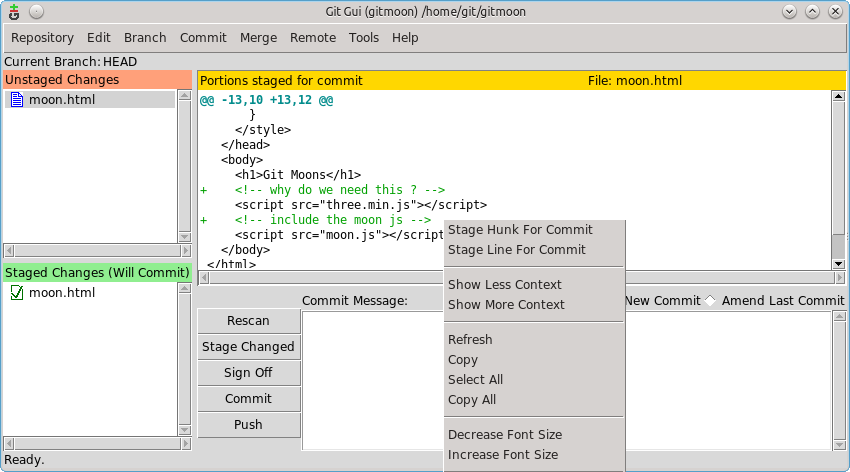
\includegraphics[width=10.5cm]{../screen/git-gui.png}}
  \subslidetitle
\end{frame}

\subsection{Textmode Interface for git - tig}
\begin{frame}[fragile]
  \subslidetitle
  The program \cmd{tig} displays the history and allows to control git interactively:
  \\
  \vspace{1em}
  \centerline{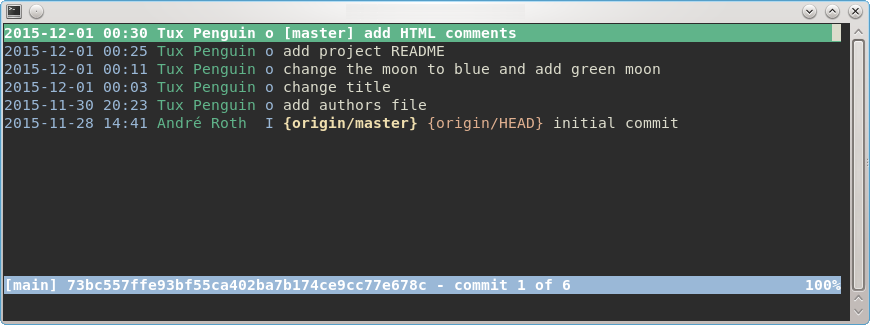
\includegraphics[width=10.5cm]{../screen/tig.png}}

  \vspace{1em}
  Note: Press \cmd{q} to quit, or \cmd{h} for help.
\end{frame}

\subsection{gitk}
\begin{frame}[fragile]
  \subslidetitle
  The program \cmd{gitk} allows to display and control git commits in a GUI:
  \\
  \vspace{1em}
  \centerline{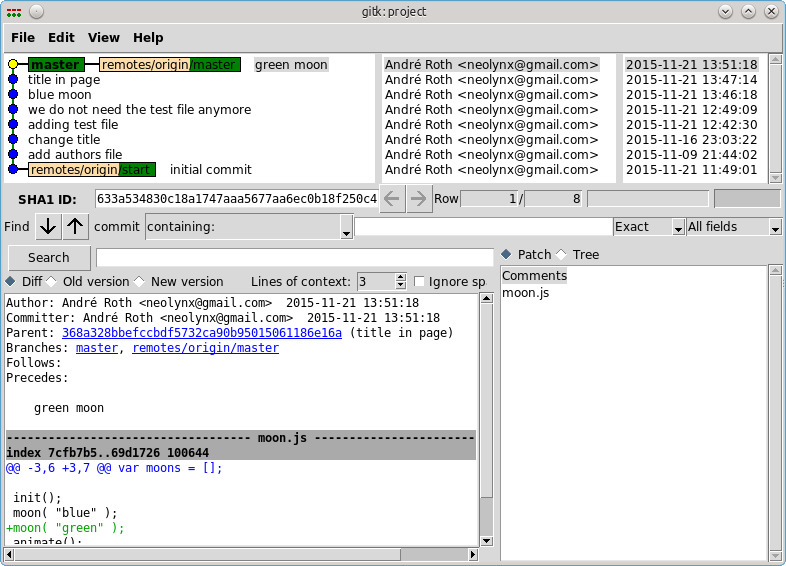
\includegraphics[width=9cm]{../screen/gitk.png}}
\end{frame}


\section{Git Branches}
\begin{frame}[fragile]
  \slidetitle

  This section covers the following topics:
  \begin{itemize}
    \pause
    \item Create and delete branches
    \pause
    \item Work with branches
    \pause
    \item Rebase branches
    \pause
    \item Merge branches
  \end{itemize}
\end{frame}

\subsection{The master branch}
\begin{frame}[fragile]
  \subslidetitle

  With git, you are always working on a branch and the default git branch is called \cmd{master}.
  \newline \vspace{1em}
  \centerline{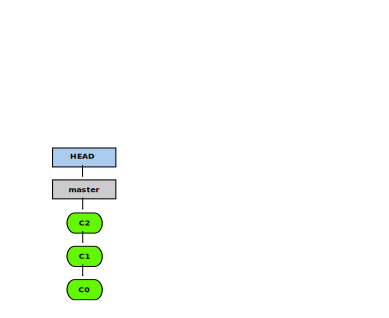
\includegraphics{diagrams/branch-master.pdf}}

  \vspace{1.2em}
  Note: \cmd{HEAD} always points to the current branch.

\end{frame}

\subsection{Creating branches}
\begin{frame}[fragile]
  \subslidetitle

  To create a new \cmd{foo} branch, append the branch name to the \cmd{git branch} command:
  \begin{lstlisting}
(*\textcolor[HTML]{18B2B2}{(master)}*) $ (*\textcolor[HTML]{0000AA}{git branch foo}*)
\end{lstlisting}

  The \cmd{git branch} command lists all your local branches:
  \begin{lstlisting}
(*\textcolor[HTML]{18B2B2}{(master)}*) $ (*\textcolor[HTML]{0000AA}{git branch}*)
  foo
* (*\textcolor[HTML]{00AA00}{master}*)
\end{lstlisting}

  \vspace{1em}
  Note: The branch you are currently on is marked with an asterisk (*).
\end{frame}

\subsection{Switching to branch}
\begin{frame}[fragile]
  \subslidetitle
  The \cmd{git checkout} command is used to change the current branch:
  \begin{lstlisting}
(*\textcolor[HTML]{18B2B2}{(master)}*) $ (*\textcolor[HTML]{0000AA}{git checkout foo}*)
Switched to branch 'foo'

(*\textcolor[HTML]{18B2B2}{(foo)}*) $ (*\textcolor[HTML]{0000AA}{git branch}*)
* (*\textcolor[HTML]{00AA00}{foo}*)
  master
\end{lstlisting}

  \vspace{1em}
  The \cmd{git checkout} command with \cmd{-b} option creates a new branch and automatically switches to it:
  \begin{lstlisting}
(*\textcolor[HTML]{18B2B2}{(foo)}*) $ (*\textcolor[HTML]{0000AA}{git checkout -b bar}*)
Switched to a new branch 'bar'

(*\textcolor[HTML]{18B2B2}{(bar)}*) $ (*\textcolor[HTML]{0000AA}{git branch}*)
* (*\textcolor[HTML]{00AA00}{bar}*)
  foo
  master
\end{lstlisting}
\end{frame}

\subsection{Deleting a branch}
\begin{frame}[fragile]
  \subslidetitle
  To delete an existing branch use the \cmd{-d} or \cmd{-D} (force) flag:
\begin{lstlisting}
(*\textcolor[HTML]{18B2B2}{(bar)}*) $ (*\textcolor[HTML]{0000AA}{git checkout master}*)

(*\textcolor[HTML]{18B2B2}{(master)}*) $ (*\textcolor[HTML]{0000AA}{git branch -d foo bar}*)
Deleted branch foo (was c974445).
Deleted branch bar (was 9adadac).

(*\textcolor[HTML]{18B2B2}{(master)}*) $ (*\textcolor[HTML]{0000AA}{git branch}*)
* (*\textcolor[HTML]{00AA00}{master}*)
\end{lstlisting}

  \vspace{1em}
  Note: you cannot delete the branch you are currently working on.
\end{frame}

\subsection{Rebasing}
\begin{frame}[fragile]
  \subslidetitle
  Rebase puts a branch on top of an other:
  \centerline{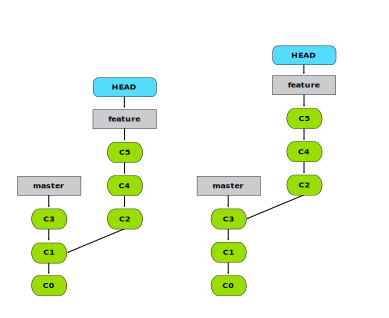
\includegraphics{diagrams/branch-rebase.pdf}}
\end{frame}

\subsection{Prepare for rebase exercise}
\begin{frame}[fragile]
  \subslidetitle

  Start to create a new fix-title branch:
  \begin{lstlisting}
(*\textcolor[HTML]{18B2B2}{(master)}*) $ (*\textcolor[HTML]{0000AA}{git checkout -b fix-title}*)
Switched to a new branch 'fix-title'
\end{lstlisting}

  Modify the \cmd{moon.html} according to this diff instructions:
  \begin{lstlisting}
(*\textcolor[HTML]{18B2B2}{@@ -7,7 +7,8 @@}*)
        font-family: Monospace;
(*\textcolor[HTML]{AA0000}{-}*)        (*\textcolor[HTML]{AA0000}{background-color: \#f0f0f0; <!-- grey -->}*)
(*\textcolor[HTML]{00AA00}{+}*)        (*\textcolor[HTML]{00AA00}{background-color: black;}*)
(*\textcolor[HTML]{00AA00}{+}*)        (*\textcolor[HTML]{00AA00}{color: white;}*)
        margin: 0px;
\end{lstlisting}
\end{frame}

\subsection{Prepare for rebase exercise}
\begin{frame}[fragile]
  \subslidetitle
  Commit your changes:
  \begin{lstlisting}
(*\textcolor[HTML]{18B2B2}{(fix-title)}*) $ (*\textcolor[HTML]{0000AA}{git commit -a -m "change title background color"}*)
\end{lstlisting}

  image
\end{frame}

\subsection{Display difference between branches}
\begin{frame}[fragile]
  \subslidetitle

  As git has the complete history locally, we can easily display changes between branches:

  \begin{lstlisting}
(*\textcolor[HTML]{18B2B2}{(fix-title)}*) $ (*\textcolor[HTML]{0000AA}{git diff master}*)
diff --git a/moon.html b/moon.html
index 145cfff..ae7bc15 100644
--- a/moon.html
+++ b/moon.html
(*\textcolor[HTML]{18B2B2}{@@ -7,7 +7,8 @@}*)
   <style>
     body {
         font-family: Monospace;
(*\textcolor[HTML]{AA0000}{-}*)         (*\textcolor[HTML]{AA0000}{background-color: \#f0f0f0; <!-- grey -->}*)
(*\textcolor[HTML]{00AA00}{+}*)         (*\textcolor[HTML]{00AA00}{background-color: black;}*)
(*\textcolor[HTML]{00AA00}{+}*)         (*\textcolor[HTML]{00AA00}{color: white;}*)
         margin: 0px;
         overflow: hidden;
     }
\end{lstlisting}
\end{frame}

\subsection{Prepare for rebase exercise}
\begin{frame}[fragile]
  \subslidetitle

  In the meantime, we need to update the README file with a Prerequisites sub-section:
  \begin{lstlisting}
(*\textcolor[HTML]{18B2B2}{(fix-title)}*) $ (*\textcolor[HTML]{0000AA}{git checkout master}*)
Switched to branch 'master'
Your branch is up-to-date with 'origin/master'.

(*\textcolor[HTML]{18B2B2}{(master)}*) $ (*\textcolor[HTML]{0000AA}{echo "\#\# Prerequisites" >> README}*)

(*\textcolor[HTML]{18B2B2}{(master)}*) $ (*\textcolor[HTML]{0000AA}{git commit -a -m "document prerequisites"}*)
\end{lstlisting}

\end{frame}

\subsection{Graphic display in gitk}
\begin{frame}[fragile]
  \subslidetitle

  Now we can see the graphical representation of our fix-title branch with \cmd{gitk}:
  \begin{lstlisting}
  (*\textcolor[HTML]{18B2B2}{(master)}*) $ (*\textcolor[HTML]{0000AA}{gitk}*)
\end{lstlisting}

  \vspace{1em}

  \centerline{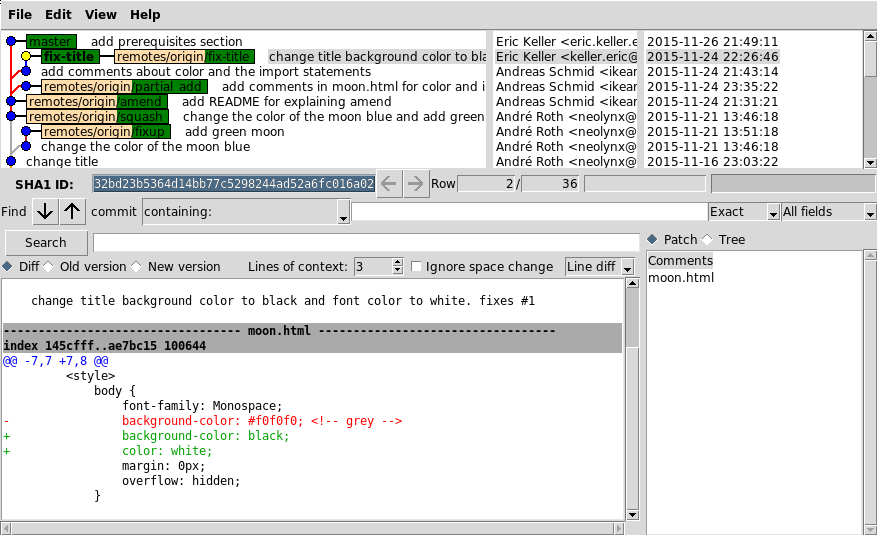
\includegraphics[width=10cm]{../screen/gitk-fix-title.png}}

\end{frame}

% rebase with master
\subsection{Rebasing a branch}
\begin{frame}[fragile]
  \subslidetitle

  Use \cmd{git rebase} to update the status of a branch on top of another branch:

  \begin{lstlisting}
(*\textcolor[HTML]{18B2B2}{(master)}*) $ (*\textcolor[HTML]{0000AA}{git checkout fix-title}*)

(*\textcolor[HTML]{18B2B2}{(fix-title)}*) $ (*\textcolor[HTML]{0000AA}{git rebase master}*)
First, rewinding head to replay your work on top of it...
Applying: add comments
Applying: change title background color
\end{lstlisting}

  As git states the rebase re-apply commits from the fix-title branches on to of the master branch.

\end{frame}

% display with tig/gitk
\subsection{Display rebase operation}
\begin{frame}[fragile]
  \subslidetitle

  Now we can see the graphical representation of our fix-title branch rebased on the master branch with \cmd{tig}:
  \begin{lstlisting}
(*\textcolor[HTML]{18B2B2}{(fix-title)}*) $ (*\textcolor[HTML]{0000AA}{tig master fix-title}*)
\end{lstlisting}

  \vspace{1em}

  \centerline{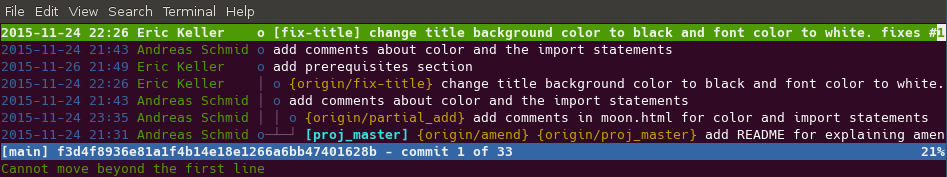
\includegraphics[width=10cm]{../screen/tig-fix-title-rebase-master.png}}

\end{frame}

\subsection{Merging}
\begin{frame}[fragile]
  \subslidetitle
  Merge integrates a branch into another:
  \centerline{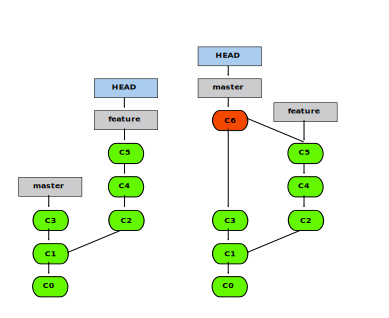
\includegraphics{diagrams/branch-merge.pdf}}
\end{frame}

\subsection{Prepare for merge exercise}
\begin{frame}[fragile]
  \subslidetitle

  A new feature request has to be implemented on from the master branch:
  \newline \vspace{1em}
  \#2 insert a white moon between the blue and green moon.
  \begin{lstlisting}
(*\textcolor[HTML]{18B2B2}{(fix-title)}*) $ (*\textcolor[HTML]{0000AA}{git checkout -b third-moon master}*)
Switched to a new branch 'third-moon'
\end{lstlisting}

  Modify the \cmd{moon.js} file following this diff instructions:
  \begin{lstlisting}
(*\textcolor[HTML]{18B2B2}{@@ -3,6 +3,7 @@}*) var moons = [];

 init();
 moon( "blue" );
(*\textcolor[HTML]{00AA00}{+}*)(*\textcolor[HTML]{00AA00}{moon( "white" );}*)
 moon( "green" );
 animate();
\end{lstlisting}
\end{frame}


\subsection{Prepare for merge exercise}
\begin{frame}[fragile]
  \subslidetitle

  Commit your changes:
  \begin{lstlisting}
(*\textcolor[HTML]{18B2B2}{(third-moon)}*) $ (*\textcolor[HTML]{0000AA}{git commit -a -m "add a white moon between the blue and green moon, implements \#2"}*)
\end{lstlisting}

\end{frame}


\subsection{Prepare for merge exercise}
\begin{frame}[fragile]
  \subslidetitle

  An emergency fix has to be done on the master branch:
  \newline \vspace{1em}
  \#3 We are not able to make it work, please specify the prerequisites
  \begin{lstlisting}
(*\textcolor[HTML]{18B2B2}{(third-moon)}*) $ (*\textcolor[HTML]{0000AA}{git checkout master}*)
Switched to branch 'master'
Your branch is up-to-date with 'origin/master'.
\end{lstlisting}

  Modify the README as following:
  \begin{lstlisting}
(*\textcolor[HTML]{18B2B2}{(master)}*) $ (*\textcolor[HTML]{0000AA}{echo "}*)
> (*\textcolor[HTML]{0000AA}{use webgl browser" >> README}*)
\end{lstlisting}

  Commit your changes:
  \begin{lstlisting}
(*\textcolor[HTML]{18B2B2}{(master)}*) $ (*\textcolor[HTML]{0000AA}{git commit -a -m "update prerequisites subsection"}*)
\end{lstlisting}

\end{frame}
\subsection{Before merge}
\begin{frame}[fragile]
  \subslidetitle

  Now we can see the graphical representation of our third-moon branch \cmd{tig}:
  \begin{lstlisting}
(*\textcolor[HTML]{18B2B2}{(master)}*) $ (*\textcolor[HTML]{0000AA}{tig master third-moon}*)
\end{lstlisting}

  \vspace{1em}

  \centerline{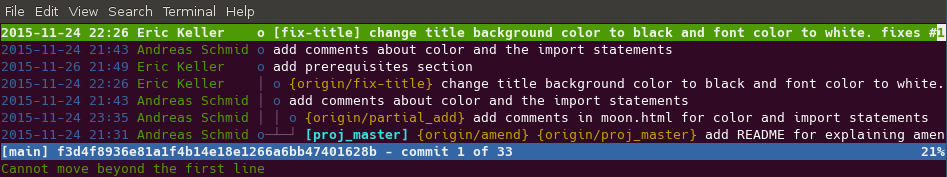
\includegraphics[width=10cm]{../screen/tig-fix-title-rebase-master.png}}

\end{frame}


\subsection{Merging a branch}
\begin{frame}[fragile]
  \subslidetitle

  Use \cmd{git merge} to merge a branch into another branch:

  \begin{lstlisting}
(*\textcolor[HTML]{18B2B2}{(master)}*) $ (*\textcolor[HTML]{0000AA}{git merge third-moon}*)
Merge branch 'third-moon' into master

# Please enter a commit message to explain why this merge is necessary,
# especially if it merges an updated upstream into a topic branch.
#
# Lines starting with '#' will be ignored, and an empty message aborts
# the commit.
\end{lstlisting}


\end{frame}

\subsection{After merge}
\begin{frame}[fragile]
  \subslidetitle

  Now we can see the graphical representation of our third-moon branch merged on the master branch with \cmd{tig}:
  \begin{lstlisting}
(*\textcolor[HTML]{18B2B2}{(master)}*) $ (*\textcolor[HTML]{0000AA}{tig master third-moon}*)
\end{lstlisting}

  \vspace{1em}

  \centerline{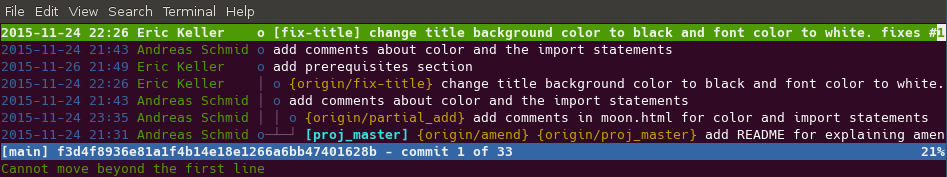
\includegraphics[width=10cm]{../screen/tig-fix-title-rebase-master.png}}

\end{frame}

\subsection{Make a tag}
\begin{frame}[fragile]
  \subslidetitle

  Let\'s make a tag:
  \begin{lstlisting}
(*\textcolor[HTML]{18B2B2}{(master)}*) $ (*\textcolor[HTML]{0000AA}{git tag v1.0.0}*)
\end{lstlisting}

\end{frame}


% git checkout branch which was edited a long time ago, and we can continue to edit at this stage.

\section{Handling merge conflicts}
\begin{frame}[fragile]
    \slidetitle
  In this section you will learn to handle conflicts with:
  \begin{itemize}
\item difftool
\item mergetool
\item 3 way merge
\end{itemize}
\end{frame}

\subsection{A requirement change}
\begin{frame}[fragile]
    \subslidetitle
  Our customer changed his mind about the color of the green moon.
  \newline \vspace{1em}
  \#4 Change the color of the green moon to red.

  Implement the change in moon.js following this diff:
\begin{lstlisting}
(*\textcolor[HTML]{18B2B2}{@@ -4,7 +4,7 @@}*) var moons = [];
 init();
 moon( "blue" );
 moon( "white" );
(*\textcolor{red}{-}*)(*\textcolor{red}{moon( "green" );}*)
(*\textcolor[HTML]{00AA00}{+}*)(*\textcolor[HTML]{00AA00}{moon( "red" );}*)
 animate();
\end{lstlisting}

\end{frame}

\subsection{Display differences}
\begin{frame}[fragile]
    \subslidetitle
  The \cmd{git difftool} will run the application of your choice to display differences:
  \begin{lstlisting}
(*\textcolor[HTML]{18B2B2}{(master)}*) $ (*\textcolor[HTML]{0000AA}{git difftool --tool kdiff3}*)
Viewing (1/1): 'moon.js'
Launch 'kdiff3' [Y/n]: Y
\end{lstlisting}

  \vspace{1em}
  \centerline{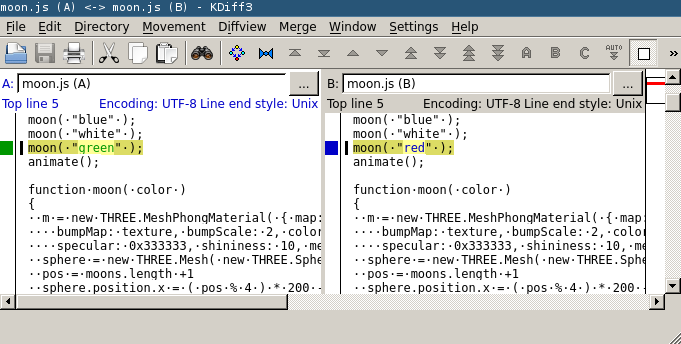
\includegraphics[width=10cm]{../screen/git-difftool-kdiff3.png}}

  Note: This can be helpful to call an external diff toll like kdiff3 or meld, especially to have a side-by-side diff.

\end{frame}


\subsection{Update feature-flag-color}
\begin{frame}[fragile]
    \subslidetitle
  Commit your changes on master:
\begin{lstlisting}
(*\textcolor[HTML]{18B2B2}{(master)}*) $ (*\textcolor[HTML]{0000AA}{git commit -a -m "change the green moon color to red, implements \#4"}*)
(*\textcolor[HTML]{18B2B2}{(master)}*) $ (*\textcolor[HTML]{0000AA}{git checkout feature-color-flag}*)
\end{lstlisting}

  Add a comment to the green moon like defined in the following diff:
  \begin{lstlisting}
(*\textcolor[HTML]{18B2B2}{@@ -4,7 +4,7 @@}*) var moons = [];
 init();
 moon( "blue" );
 moon( "white" );
(*\textcolor{red}{-}*)(*\textcolor{red}{moon( "green" );}*)
(*\textcolor[HTML]{00AA00}{+}*)(*\textcolor[HTML]{00AA00}{moon( "green" ); // no requirement}*)
 animate();
\end{lstlisting}

  Commit your changes:
  \begin{lstlisting}
(*\textcolor[HTML]{18B2B2}{(master)}*) $ (*\textcolor[HTML]{0000AA}{git commit -a -m "add comment about requirement for the green color"}*)
\end{lstlisting}
\end{frame}

\subsection{Merge feature-flag-color}
\begin{frame}[fragile]
    \subslidetitle

  The feature-flag-color is ready to be merged to master, try to merge the feature-flag-color branch to master:
\begin{lstlisting}
(*\textcolor[HTML]{18B2B2}{(feature-flag-color)}*) $ (*\textcolor[HTML]{0000AA}{git checkout master}*)
Switched to branch 'master'
Your branch is up-to-date with 'origin/master'.
(*\textcolor[HTML]{18B2B2}{(master)}*) $ (*\textcolor[HTML]{0000AA}{git merge feature-flag-color}*)
Auto-merging moon.js
CONFLICT (content): Merge conflict in moon.js
Automatic merge failed; fix conflicts and then commit the result.
\end{lstlisting}

Here we go, our first conflict, keep calm, and use \cmd{git mergetool}

\end{frame}

\subsection{Resolve a conflict}
\begin{frame}[fragile]
    \subslidetitle
\end{frame}

\subsection{Three way merge}
\begin{frame}[fragile]
    \subslidetitle
\end{frame}

\subsection{git difftool}
\begin{frame}[fragile]
    \subslidetitle
\end{frame}


\section{Git remotes}
\begin{frame}[fragile]
  \slidetitle
  This section covers the following topics:
  \begin{itemize}
    \item Git remote repository concept
    \item Add remote repositories
    \item Synchronize with remote repositories
  \end{itemize}
\end{frame}

\subsection{Remote repositories}
\begin{frame}[fragile]
  \subslidetitle
  The \cmd{git remote} allows to manage remote repositories:
  \begin{lstlisting}
$ (*\textcolor[HTML]{0000AA}{git remote show}*)
origin

$ (*\textcolor[HTML]{0000AA}{git remote show origin}*)
* remote origin
  Fetch URL: https://github.com/neolynx/gitmoon.git
  Push  URL: https://github.com/neolynx/gitmoon.git
  HEAD branch: master
  Remote branch:
    master tracked
  Local branch configured for 'git pull':
    master merges with remote master
  Local ref configured for 'git push':
    master pushes to master (up to date)
\end{lstlisting}
  \vspace{1em}
  Note: the default remote is called \textbf{origin}
\end{frame}

\subsection{Git protocols}
\begin{frame}[fragile]
  \subslidetitle
  Git repositories can be accessed locally or over the network.
  \\
  \vspace{1em}
  Various protocols are supported:
  \begin{itemize}
  \opt{local}  {file system based}
  \opt{http[s]}{good for read only access without password}
  \opt{ssh}    {normally used for read-write access}
  \opt{git}    {git native protocol on port 9418}
  \opt{legacy} {ftp, rsync, ...}
  \end{itemize}
\end{frame}

\subsection{Configure SSH access}
\begin{frame}[fragile]
  \subslidetitle
  Create a SSH key pair:
  \begin{lstlisting}
$ (*\textcolor[HTML]{0000AA}{ssh-keygen}*)
Generating public/private rsa key pair.
Enter file in which to save the key (...): (*\textcolor[HTML]{0000AA}{<enter>}*)
Created directory '.../.ssh'.
Enter passphrase (empty for no passphrase): (*\textcolor[HTML]{0000AA}{<enter>}*)
Enter same passphrase again: (*\textcolor[HTML]{0000AA}{<enter>}*)
Your identification has been saved in .../.ssh/id_rsa.
Your public key has been saved in .../.ssh/id_rsa.pub.
The key fingerprint is:
7e:f8:15:2a:b3:a2:9c:30:4e:c7:60:50:a4:d5:a9:82 user@host
The key's randomart image is:
+--[ RSA 2048]----+
|   . . .         |
|  . = = S        |
|   = X * X O o   |
...
\end{lstlisting}
\end{frame}

\subsection{Configure SSH access}
\begin{frame}[fragile]
  \subslidetitle
  Display your public key:
  \begin{lstlisting}
$ (*\textcolor[HTML]{0000AA}{cat \textasciitilde/.ssh/id\_rsa.pub}*)
ssh-rsa AAAAB3NzaC1yc2EAAAADAQABAAABAQDOmt7Y4H51gc2m
GmZsFzES6shVLFLEJ/lFCTwyosWHYDaluK71nGCelp61oTocgf4N
HBwTZmo0EZ1k0RHYt8Q3LF8e5fbC+dXt5E35XtkVFuUC7IG2/6fm
NW41j3lw9UUVrOBDgx+QvvoCuRQaxNd4mRaLsRbj9WXt17hGuNNW
ioKPWLSpw/4KHJ34hCrnliAQJ+jlW/0ieOooFp057diCka6Jn7BW
jXHi8sWMxIfyPyV2+4Kt8OpChFNYjzaL5LMRRhMnvJ8zP5SFJB2q
HP50zPYQ+gKoSda7GZedZRgD7gT7ir/u8X9HSpNyTNTafhp9+3Aj
uUiYLTgtczTgYk/T user@host
\end{lstlisting}

  This whole output can be added to the SSH access keys
  section in the web front end of your git appliance.
\end{frame}

\subsection{Exercises}
\begin{frame}[fragile]
  \subslidetitle
  Create a commit for each exercise below:
  \begin{exercise}
    \item Create a SSH key pair
    \item Configure SSH access in your git appliance
    \item Create a new private repository, called \textbf{mygitmoon}
    \item Clone the private repository in your home \\
      (Hint: switch to your home directory first, by typing \cmd{cd})
    \item Go back to the original gitmoon project (\cmd{cd \textasciitilde/gitmoon})
  \end{exercise}
\end{frame}

\subsection{Adding a remote repository}
\begin{frame}[fragile]
  \subslidetitle
  Let's add the private repository as remote \textbf{upstream}:
  \begin{lstlisting}
$ (*\textcolor[HTML]{0000AA}{git remote add upstream} \textcolor[HTML]{444444}{URL}*)
$ (*\textcolor[HTML]{0000AA}{git remote show}*)
origin
upstream
\end{lstlisting}
\end{frame}

\subsection{Pushing commits to a remote}
\begin{frame}[fragile]
  \subslidetitle
  Now, we can push our local commits to the \textbf{upstream} remote:
  \begin{lstlisting}
$ (*\textcolor[HTML]{0000AA}{git push upstream master}*)
git push upstream master
Counting objects: 6, done.
Delta compression using up to 2 threads.
Compressing objects: 100% (6/6), done.
Writing objects: 100% (6/6), 331.07 KiB | 0 bytes/s, done.
Total 6 (delta 0), reused 0 (delta 0)
remote: ...
To (*\textcolor[HTML]{444444}{URL}*)
 * [new branch]      master -> master
\end{lstlisting}
\end{frame}

\subsection{Pulling commits from a remote}
\begin{frame}[fragile]
  \subslidetitle
  In our \textbf{mygitmoon} project, these commits can now be pulled:
  \begin{lstlisting}
$ (*\textcolor[HTML]{0000AA}{cd \textasciitilde/mygitmoon}*)
$ (*\textcolor[HTML]{0000AA}{git pull}*)
remote: Counting objects: 6, done.
remote: Compressing objects: 100% (6/6), done.
remote: Total 6 (delta 0), reused 0 (delta 0)
Unpacking objects: 100% (6/6), done.
From (*\textcolor[HTML]{444444}{URL}*)
 * [new branch]      master     -> origin/master
\end{lstlisting}
\end{frame}

\subsection{git fetch}
\begin{frame}[fragile]
  \subslidetitle
\end{frame}

\subsection{Stashing modifications}
\begin{frame}[fragile]
  \subslidetitle

  Imagine you are in the middle of a modification.

  \begin{lstlisting}
$ (*\textcolor[HTML]{0000AA}{git status}*)
...
       (*\textcolor[HTML]{AA0000}{modified:   AUTHORS}*)
...
\end{lstlisting}

  And suddenly something really important needs to be done immediately!

  \begin{lstlisting}
$ (*\textcolor[HTML]{0000AA}{git stash}*)
Saved working directory and index state WIP on master: a7281d1 add authors file
HEAD is now at a7281d1 add authors file
$ (*\textcolor[HTML]{0000AA}{git status}*)
# On branch master
nothing to commit (working directory clean)
\end{lstlisting}
  Note: you now have a clean working directory again.
\end{frame}


\subsection{Restore changes}
\begin{frame}[fragile]
  \subslidetitle

  Do not worry, \textbf{git stash} does not loose any information, let's have a look:

  \begin{lstlisting}
$ (*\textcolor[HTML]{0000AA}{git stash list}*)
stash@{0}: WIP on master: a7281d1 add authors file
(END)
\end{lstlisting}

  Restore the changes from the stash queue:

  \begin{lstlisting}
$ (*\textcolor[HTML]{0000AA}{git stash pop}*)
On branch master
Changes not staged for commit:
   (use "git add <file>..." to update what will be committed)
   (use "git checkout -- <file>..." to discard changes in working directory)

       (*\textcolor[HTML]{AA0000}{modified:}*)   (*\textcolor[HTML]{AA0000}{AUTHORS}*)

no changes added to commit (use "git add" and/or "git commit -a")
Dropped refs/stash@{0} (1638e645e67ff57ffc76b2c79f851ec894ddd74c)
\end{lstlisting}
\end{frame}

\subsection{git remote update}
\begin{frame}[fragile]
  \subslidetitle
  ??
\end{frame}

\subsection{Forking a repository}
\begin{frame}[fragile]
  \subslidetitle
  A git appliance usually offers to fork a project.\\
  Forking means to create a linked copy of a git repository.
  \vspace{1em}
  This is useful for:
  * working on repositories you have no write access
  * creating pull requests
\end{frame}

\subsection{Creating a pull request}
\begin{frame}[fragile]
  \subslidetitle
\end{frame}

\subsection{Branching models}
\begin{frame}[fragile]
  \subslidetitle
\end{frame}

\section{Work with pull requests}
\begin{frame}[fragile]
    \slidetitle
\end{frame}


\section{Extras}
\begin{frame}[fragile]
  \slidetitle
\end{frame}

\subsection{Work with patches}
\begin{frame}[fragile]
    \subslidetitle
\end{frame}

\subsection{git format-patch}
\begin{frame}[fragile]
    \subslidetitle
\end{frame}

\subsection{git am}
\begin{frame}[fragile]
    \subslidetitle
\end{frame}

\subsection{Configure git}
\begin{frame}[fragile]
  \subslidetitle
  \begin{block}{Getting started with git}
    Once you have git installed you are able to configure git on 3 different levels:
    \begin{itemize}
      \option{local repository level}{path/to/repository/.git/config}
      \option{user level}{ /home/\$USER/.gitconfig }
      \option{system level}{on GNU/Linux: /etc/gitconfig}
    \end{itemize}

    The configuration file is a simple text file and can be edited with any text editor.
    Priority of git config: local, user, system.
  \end{block}
\end{frame}

\subsection{git config}
\begin{frame}[fragile]
  \subslidetitle
  The command \cmd{git config} can be used to change the global, system and local config of git.
  \begin{itemize}
      \option{git config ..}{}
      \option{git config --global ..}{}
      \option{git config --system ..}{}
  \end{itemize}
\end{frame}

\subsection{Set username and email}
\begin{frame}[fragile]
  \subslidetitle
  \vspace{1em}
  Set your name and email locally:
  \begin{itemize}
      \option{git config add user.name "My name"}{}
      \option{git config add user.email "myemail@git.ch"}{}
  \end{itemize}
  \vspace{1em}
  Or globally:
  \begin{itemize}
      \option{git config --global add user.name "My name"}{}
      \option{git config --global add user.email "myemail@git.ch"}{}
  \end{itemize}

  Extract from \bf{$\sim$/.gitconfig}
\begin{lstlisting}
[user]
  name = Andreas Schmid
  email = ikeark@gmail.com
\end{lstlisting}
\end{frame}

\subsection{Create aliases}
\begin{frame}[fragile]
  \subslidetitle

  Git allows to create aliases for commands.

  Example:

  instead of typing \bf{git status} we want to type \bf{git st}.

  Define alias:
  \begin{lstlisting}
  git config --global alias.st = status
  git config --global alias.co = checkout
  git config --global alias.ci = commit
  git config --global alias.br = branch
  \end{lstlisting}


  Extract from \bf{$\sim$/.gitconfig}
\begin{lstlisting}
[alias]
  st = status
  co = checkout
  ci = commit
  br = branch
  l = log --graph --pretty=format:'%C(yellow)%h%C(cyan)%d%Creset %s %C(white)- %an, %ar%Creset'
  ll = log --stat --abbrev-commit
\end{lstlisting}
\end{frame}

\subsection{Set mergetool}
\begin{frame}[fragile]
  \subslidetitle
\begin{lstlisting}
[merge]
  tool = kdiff3
\end{lstlisting}
\end{frame}

\subsection{Example $\sim$/.gitconfig}
\begin{frame}[fragile]
  \subslidetitle

\begin{lstlisting}
[user]
  name = Andreas Schmid
  email = ikeark@gmail.com

[color]
  diff = auto
  status = auto
  branch = auto
  grep = auto

[alias]
  st = status
  co = checkout
  ci = commit
  br = branch
  l = log --graph --pretty=format:'%C(yellow)%h%C(cyan)%d%Creset %s %C(white)- %an, %ar%Creset'
  ll = log --stat --abbrev-commit

[merge]
  tool = kdiff3
\end{lstlisting}
\end{frame}
\subsection{git bash prompt}
\begin{frame}[fragile]
  \subslidetitle

  Don't you like this bash prompt:
  \begin{lstlisting}
  (*\textcolor[HTML]{54FF54}{kraeki@deathstar:}*)(*\textcolor[HTML]{5454FF}{\textasciitilde/work/gitworkshop}*) (*\textcolor[HTML]{18B2B2}{(master)}*) $
  (*\textcolor[HTML]{54FF54}{kraeki@deathstar:}*)(*\textcolor[HTML]{5454FF}{\textasciitilde/work/gitworkshop}*) (*\textcolor[HTML]{18B2B2}{(master)}*) $
  \end{lstlisting}

  In your \cmd{\textasciitilde/.bashrc} replace your prompt with this:
  In your \cmd{\textasciitilde/.bashrc} replace your prompt with this:
  \begin{lstlisting}[language=bash]
GIT_PS1_SHOWDIRTYSTATE=1 # showing state of working directory
color_prompt=yes
if [ "$color_prompt" = yes ]; then
  PS1='${debian_chroot:+($debian_chroot)}\[\033[00m\]\[\033[01;32m\]\u@\h\[\033[00m\]:\[\033[01;34m\]\w\[\033[00m\]\[\033[0;36m\]$(__git_ps1 " (%s)")\[\033[00m\] \$ '
else
  PS1='${debian_chroot:+($debian_chroot)}\u@\h:\w\$ '
fi
unset color_prompt force_color_prompt
\end{lstlisting}

  Don't forget to reload your bash environment: \cmd{source \textasciitilde/.bashrc}
  Don't forget to reload your bash environment: \cmd{source \textasciitilde/.bashrc}

\end{frame}



\end{document}

